\documentclass[11pt]{article}
\usepackage{amsmath,amssymb,amsthm}
\usepackage[margin=1.05in]{geometry}
\usepackage{booktabs}
\usepackage{array}
\usepackage{graphicx}
\usepackage{microtype}
\usepackage[colorlinks=true,linkcolor=blue,citecolor=blue,urlcolor=blue]{hyperref}
\usepackage{xurl}
\hypersetup{pdftitle={Exact-arithmetic certificates for three autoconvolution
  inequalities},pdfauthor={Kevin Russell (ProjectForty2 / CHRONOS agent)}}

\newtheorem{theorem}{Theorem}
\newtheorem{lemma}[theorem]{Lemma}
\newtheorem{proposition}[theorem]{Proposition}
\theoremstyle{remark}
\newtheorem{remark}[theorem]{Remark}

\newcommand{\NN}{\mathbb{N}}
\newcommand{\RR}{\mathbb{R}}
\newcommand{\ZZ}{\mathbb{Z}}
\newcommand{\supnorm}[1]{\lVert #1 \rVert_\infty}
\newcommand{\onenorm}[1]{\lVert #1 \rVert_1}
\newcommand{\twonorm}[1]{\lVert #1 \rVert_2}

\title{Exact-arithmetic certificates for three autoconvolution
inequalities,\\ with machine-verified re-evaluations of four published
constructions}
\author{Kevin Russell\thanks{%
Correspondence: \texttt{kevinrussell@gmail.com}. Computer-assisted note,
prepared with CHRONOS, ProjectForty2's autonomous research agent; the author
takes responsibility for all claims. The three \emph{constructions} certified
here are due to the agents ``Hyra'' (Theorems~\ref{thm:c1} and~\ref{thm:c2})
and ``OrganonAgent'' (Theorem~\ref{thm:c3}) on the EinsteinArena platform
\cite{Hyra26,Organon26}; see the attribution statement in
Section~\ref{sec:intro}. Verification artifacts are listed in
Appendix~\ref{sec:repro}.}\\[3pt]
{\normalsize ProjectForty2 --- CHRONOS agent}}
\date{July 4, 2026}

\begin{document}
\maketitle

\begin{abstract}
We give machine-verified, exact-rational-arithmetic bounds for the three
autoconvolution inequality constants popularized by the recent AI-search
literature. Writing $g = f * f$ for the autoconvolution, the constants are
$C_1$ (the least possible $\sup_t g$ for nonnegative $f$ supported on
$[-\tfrac14,\tfrac14]$ with $\int f = 1$), $C_2$ (the largest possible
$\twonorm{g}^2 / (\onenorm{g}\,\supnorm{g})$ for nonnegative $f$), and $C_3$
(the signed-$f$ analogue of $C_1$). We prove
\[
C_1 \le Q_1 < 1.5028503020710078765191888, \qquad
C_2 \ge Q_2 > 0.9629011010961756912885013,
\]
\[
C_3 \le Q_3 < 1.452304333183157960701885,
\]
where $Q_1, Q_2, Q_3$ are explicit rational numbers, obtained by evaluating
exactly the functionals of three explicit step-function constructions found
by AI search agents on the EinsteinArena platform. A short lemma shows that
for a step function the autoconvolution is piecewise linear with breakpoints
on the half-grid, so the continuum supremum and the $L^1$, $L^2$, $L^\infty$
norms are finite exact computations, with zero discretization loss; the
evaluations are carried out in exact integer arithmetic (Kronecker-substitution
convolution up to $n = 524288$ cells) with no floating-point operation on any
certified path. For $C_1$ this is, to our knowledge, the first
exact-arithmetic-certified upper bound in the sub-$1.51$ regime (the best
previous fully proven value being the classical $\pi/2$); for $C_3$ it is, to
our knowledge, the first rigorously certified nontrivial upper bound for the
signed variant. We additionally re-certify, exactly, four published
construction vectors --- Matolcsi--Vinuesa, AlphaEvolve, Boyer--Li, and
Jaech--Joseph --- upgrading three float reports to theorem grade
(Jaech--Joseph for $C_2$, Matolcsi--Vinuesa and AlphaEvolve for $C_3$),
independently confirming the Boyer--Li exact fraction, correcting a misstated
$\infty$-norm claim of Matolcsi--Vinuesa, and repairing two points of
citation hygiene in this literature. These certificates evaluate existing
arena leader vectors: they tie, and do not beat, the corresponding
floating-point leaderboard scores; the contribution is that float records
become theorems. Items not machine-verified at the time of writing are
listed in a pending-verification ledger.
\end{abstract}

\medskip
\noindent\textbf{MSC 2020:} 42A85 (primary); 26D15, 11B75, 65G30
(secondary).\\
\textbf{Keywords:} autoconvolution inequalities; computer-assisted proof;
exact rational arithmetic; Kronecker substitution; certification of numerical
records.

\section{Introduction}\label{sec:intro}

Let $f * f$ denote the autoconvolution
$(f*f)(t) = \int_\RR f(t-x) f(x)\,dx$. Three extremal constants for
autoconvolutions have become standard
benchmarks in the recent literature on AI-driven mathematical search
\cite{AlphaEvolve25,MathScale25,ThetaEvolve25,TTT26,SimpleTES26}, following a
much older analytic tradition
\cite{SS02,MO09,MV10,CS17}:

\begin{itemize}
\item[$(C_1)$] the \emph{first autocorrelation inequality}: the largest
constant $C_1$ with
\[
\max_{t}\, (f*f)(t) \;\ge\; C_1 \Bigl(\int f\Bigr)^{2}
\qquad\text{for all } f \ge 0 \text{ supported on } [-\tfrac14,\tfrac14].
\]
Equivalently $C_1 = \inf_f \sup_t (f*f)(t)$ over nonnegative $f$ supported on
$[-\tfrac14,\tfrac14]$ with $\int f = 1$. This is the constant of Schinzel
and Schmidt \cite{SS02}, studied by Martin--O'Bryant \cite{MO09},
Matolcsi--Vinuesa \cite{MV10}, and Cloninger--Steinerberger \cite{CS17}; it
is Problem~6.2 of \cite{MathScale25}.
\item[$(C_2)$] the \emph{second autocorrelation inequality}: the smallest
constant $C_2$ with
\[
\twonorm{f*f}^{2} \;\le\; C_2\, \onenorm{f*f}\, \supnorm{f*f}
\qquad\text{for all } f \ge 0,\; f \in L^1 \cap L^2 ,
\]
i.e.\ $C_2 = \sup_f \twonorm{f*f}^2/(\onenorm{f*f} \supnorm{f*f})$, a
question of Martin and O'Bryant \cite{MO09}; the ratio is scale- and
dilation-invariant, so no support normalization is needed. This is
Problem~6.3 of \cite{MathScale25}.
\item[$(C_3)$] the \emph{third autocorrelation inequality}: the signed
variant of $(C_1)$, the largest constant $C_3$ with
\[
\Bigl|\max_{-\frac12 \le t \le \frac12} (f*f)(t)\Bigr| \;\ge\;
C_3 \Bigl(\int f\Bigr)^{2}
\qquad\text{for all } f\colon [-\tfrac14,\tfrac14] \to \RR,\ \int f \neq 0 ,
\]
where $f$ \emph{may take negative values}. This is the constant
$C'_{6.4}$ of \cite[Problem 6.4(b)]{MathScale25}; the earliest example we
know of is the closing remark of Matolcsi--Vinuesa \cite{MV10}. (The
absolute value is in fact inert: $\max_t (f*f)(t) \ge (\int f)^2 > 0$ for
every admissible $f$, by the averaging argument of
Remark~\ref{rem:c3lower}.)
\end{itemize}

\paragraph{Status before this note.} For $C_1$, the best \emph{proven}
upper bound was, to our knowledge, the classical analytic value
$C_1 \le \pi/2 = 1.5707963\ldots$ of Schinzel and Schmidt \cite{SS02}, who
conjectured equality. Matolcsi and Vinuesa \cite{MV10} disproved the
conjecture by explicit computer search --- Mathematica~6 examples below
$1.522$, then LOQO solutions reaching $1.51237\ldots$, then an LP fix-point
iteration of Kolountzakis and Matolcsi reaching
$\supnorm{f*f} = 1.50972\ldots$ at $n = 208$ --- and stated the resulting
bound as $C_1 \le 1.5098$. Their printed coefficients are 8-significant-digit
decimals which, as their own remark concedes, satisfy the normalization only
up to small numerical errors, and the norm evaluations are floating point;
the same is true of every sub-$1.51$ value reported since (see
Remark~\ref{rem:c1landscape}). On the lower side, $C_1 \ge 1.28$ is the
peer-reviewed bound of Cloninger--Steinerberger \cite{CS17}; a 2026 preprint
reports an interval-certified improvement $C_1 \ge 1.2937$ \cite{KP26}.
For $C_2$, only the trivial H\"older bound $C_2 \le 1$ is known on the upper
side; on the lower (construction) side the strongest fully rigorous published
value is the exact rational of Boyer--Li \cite{BoyerLi25},
$0.90156485\ldots$, and the strongest published claim accompanied by a
released construction vector (hence independently certifiable) is the
float-evaluated $0.94136$ of Jaech--Joseph \cite{JJ25}; larger float-only
values (up to $0.9627$) have been reported by AI-search systems
\cite{MathScale25,SimpleTES26} without, to our knowledge, released vectors. For $C_3$, we are not aware of \emph{any}
previously certified nontrivial bound in either direction: the classical
example of \cite{MV10} ($1.45810\ldots$) and all subsequent reports
\cite{AlphaEvolve25,MathScale25,SimpleTES26} are floating point, and the only
known lower bound is the trivial $C_3 \ge 1$.

\paragraph{What this note proves.} Theorems~\ref{thm:c1}, \ref{thm:c2}
and~\ref{thm:c3} replace the constructive side of each of the three problems
by an explicit rational number, evaluated in exact integer arithmetic:
$C_1 \le Q_1 = 1.50285030\ldots$, $C_2 \ge Q_2 = 0.96290110\ldots$,
$C_3 \le Q_3 = 1.45230433\ldots$ Each bound is theorem-grade in the
following concrete sense: it follows from one short lemma proved here
(Lemma~\ref{lem:pwlinear}), which reduces the continuum functional of an
arbitrary step function to a finite computation with zero discretization
loss, plus a finite exact-integer-arithmetic evaluation that is fully
reproducible from the included scripts (Appendix~\ref{sec:repro}); no
floating-point quantity enters any chain. Alongside the three headline
bounds we exactly re-evaluate four published construction vectors
(Propositions~\ref{prop:c2recert} and~\ref{prop:c3recert}): this upgrades
the Jaech--Joseph $C_2$ record and the Matolcsi--Vinuesa and AlphaEvolve
$C_3$ examples from float reports to certified statements, independently
confirms the Boyer--Li fraction to the last digit, and surfaces two
corrections of record (Remarks~\ref{rem:hygiene} and~\ref{rem:mvnorm}).
Nothing in this note touches the lower bound for $C_1$, the upper bound for
$C_2$, or the lower bound for $C_3$: those sides stand exactly as published,
and are quoted, not improved.

\paragraph{Recent activity.} AI-search systems have reported (floating-point)
constructive records for all three constants: for $C_1$, AlphaEvolve reports
$1.5053$ \cite{AlphaEvolve25}, improved to $1.5032$ in the follow-up results
paper \cite{MathScale25}; ThetaEvolve reports $1.5068$ from scratch
\cite{ThetaEvolve25}; TTT-Discover reports $1.50286$ with a $30000$-piece
step function \cite{TTT26}; and a Together~AI team is tabulated at
$1.502862$ in \cite{SimpleTES26}, whose own runs report $1.503871$. For
$C_2$: $0.8962$ \cite{AlphaEvolve25}, $0.961$ \cite{MathScale25},
$0.961206$ (Together~AI, tabulated in \cite{SimpleTES26}), $0.962694$
\cite{SimpleTES26}. For $C_3$: $1.4557$ \cite{AlphaEvolve25,MathScale25},
$1.454555$ (Together~AI, tabulated in \cite{SimpleTES26}), $1.453675$
\cite{SimpleTES26}. To our knowledge none of these reports is accompanied by
an exact evaluation together with a proof that the discrete score bounds the
continuum constant --- precisely the two steps supplied below, which apply
verbatim to any step construction. Every exact value proven in this note is
on the favorable side of every float report just listed; the certification
status of the tabulated Together~AI values is unverified by us
(Section~\ref{sec:pending}), but nothing here depends on them.

\paragraph{Attribution, and what is not claimed.} This is a certification
exercise, and credit belongs where the mathematics originated. The three
step-function \emph{constructions} certified in Theorems~\ref{thm:c1},
\ref{thm:c2} and~\ref{thm:c3} were produced by anonymous AI search agents
competing on the EinsteinArena platform --- ``Hyra'' (Theorems~\ref{thm:c1}
and~\ref{thm:c2}) \cite{Hyra26} and ``OrganonAgent'' (Theorem~\ref{thm:c3})
\cite{Organon26} --- within an open ecosystem of agents iteratively
optimizing these functionals. We make no priority claim over any
construction. Our contribution is the certification lemma, the
exact-rational evaluation machinery (including Kronecker-substitution
convolution at $n = 524288$), the exact re-certifications of the
Matolcsi--Vinuesa, AlphaEvolve, Boyer--Li, and Jaech--Joseph published
vectors, and the literature corrections. We stress that the certificates
evaluate the \emph{existing} leader vectors of the arena boards: they tie,
and do not beat, the leaderboard floating-point scores (agreement is to
within a few units in the last place --- one for $C_1$ and $C_3$, four for
$C_2$ from rounding in the board verifier's FFT path, which we re-run
bit-for-bit); what changes is that three float records become theorems. This note itself was drafted and verified
computer-assisted, by CHRONOS, ProjectForty2's autonomous research agent,
operating under the author's direction; the author reviewed the mathematics
and takes full responsibility for all claims.

\section{The certification lemma}\label{sec:lemma}

Throughout, fix $n \in \NN$ and let $h = \tfrac{1}{2n}$ be the cell width of
the uniform grid on $[-\tfrac14, \tfrac14]$, with cells
$I_i = [-\tfrac14 + ih,\, -\tfrac14 + (i+1)h)$ for $0 \le i \le n-1$. Given
real (possibly negative) heights $a_0, \dots, a_{n-1}$, let
$f = \sum_i a_i \mathbf{1}_{I_i}$ and $g = f * f$. Define the discrete
autoconvolution
\[
c_m \;=\; \sum_{i+j=m} a_i a_j , \qquad m = 0, 1, \dots, 2n-2 .
\]

\begin{lemma}[step autoconvolution is piecewise linear; norms are exact]
\label{lem:pwlinear}
With the notation above:
\begin{enumerate}
\item[(i)] $g$ is continuous and piecewise linear on $\RR$, with all
breakpoints contained in the half-grid $-\tfrac12 + h\ZZ$, and $g \equiv 0$
outside $(-\tfrac12, \tfrac12)$;
\item[(ii)] the knot values are $g\bigl(-\tfrac12 + (m+1)h\bigr) = h\,c_m$
for $0 \le m \le 2n-2$, and $g(\pm\tfrac12) = 0$;
\item[(iii)] if $\sum_i a_i \neq 0$ then $\max_m c_m > 0$ and
\[
\sup_{t \in \RR} g(t) \;=\; h \max_{0 \le m \le 2n-2} c_m ,
\qquad
\supnorm{g} \;=\; h \max_{0 \le m \le 2n-2} |c_m| ;
\]
\item[(iv)] if additionally $a_i \ge 0$ for all $i$, then, exactly,
\[
\onenorm{g} \;=\; h^2 \sum_m c_m \;=\; \Bigl(\int f\Bigr)^2 ,
\qquad
\twonorm{g}^2 \;=\; \frac{h^3}{3} \sum_{m=-1}^{2n-2}
\bigl(c_m^2 + c_m c_{m+1} + c_{m+1}^2\bigr),
\]
with the zero-padding convention $c_{-1} = c_{2n-1} = 0$.
\end{enumerate}
In particular every functional appearing in $(C_1)$, $(C_2)$, $(C_3)$ is,
for a step function, a finite exact computation in the field generated by
the heights: there is zero discretization loss.
\end{lemma}

\begin{proof}
(i) By bilinearity,
$g(t) = \sum_{i,j} a_i a_j\, \lambda\bigl(I_i \cap (t - I_j)\bigr)$ with
$\lambda$ Lebesgue measure. For fixed intervals $[a,b)$ and $[c,d)$ the map
$t \mapsto \lambda\bigl([a,b) \cap (t-d,\, t-c]\bigr)$ is continuous and
piecewise linear with breakpoints in $\{a+c,\, a+d,\, b+c,\, b+d\}$; all cell
endpoints lie in $-\tfrac14 + h\ZZ$, so all breakpoints lie in
$-\tfrac12 + h\ZZ$. A finite sum of such functions is continuous piecewise
linear with breakpoints in the same lattice. Since $f$ is supported in
$[-\tfrac14,\tfrac14]$, $g$ vanishes for $|t| \ge \tfrac12$.

(ii) At $t = \tau_m := -\tfrac12 + (m+1)h$ we have
$\tau_m - I_j = \bigl(-\tfrac14 + (m-j)h,\, -\tfrac14 + (m-j+1)h\bigr]$,
which meets $I_i$ in a set of measure $h\,\delta_{i,\,m-j}$ (and measure $0$
for out-of-range indices). Hence
$g(\tau_m) = h \sum_{i+j=m} a_i a_j = h\,c_m$. At $t = \pm\tfrac12$ the
supports barely touch and $g = 0$.

(iii) A continuous piecewise-linear function on the compact interval
$[-\tfrac12,\tfrac12]$ attains its maximum at a knot or an endpoint;
endpoints give $0$, and $g \equiv 0$ outside. By Fubini,
$\int g = (\int f)^2 = h^2 (\sum_i a_i)^2 > 0$; since
$\sum_m c_m = \sum_{i,j} a_i a_j = (\sum_i a_i)^2$, some $c_m$ is strictly
positive and the maximum over knots is positive, hence dominates the
endpoint value $0$; the same knot-or-endpoint argument applied to $\pm g$
gives the $\supnorm{g}$ formula.

(iv) The trapezoid rule is exact for the piecewise-linear $g$: with zero
endpoint values, $\int g = h \sum_m g(\tau_m) = h^2 \sum_m c_m$, which equals
$(\int f)^2$ by Fubini (an internal consistency check that the implementation
verifies exactly). When $a_i \ge 0$, also $g \ge 0$, so
$\onenorm{g} = \int g = h^2 \sum_m c_m$. For $\twonorm{g}^2$, on each knot gap of
width $h$ with endpoint values $y_1, y_2$ the function is linear, and
$\int (\text{linear})^2 = \tfrac{h}{3}(y_1^2 + y_1 y_2 + y_2^2)$ exactly;
summing over the $2n$ gaps (zero-padded ends) gives the stated formula.
\end{proof}

\begin{figure}[t]
\centering
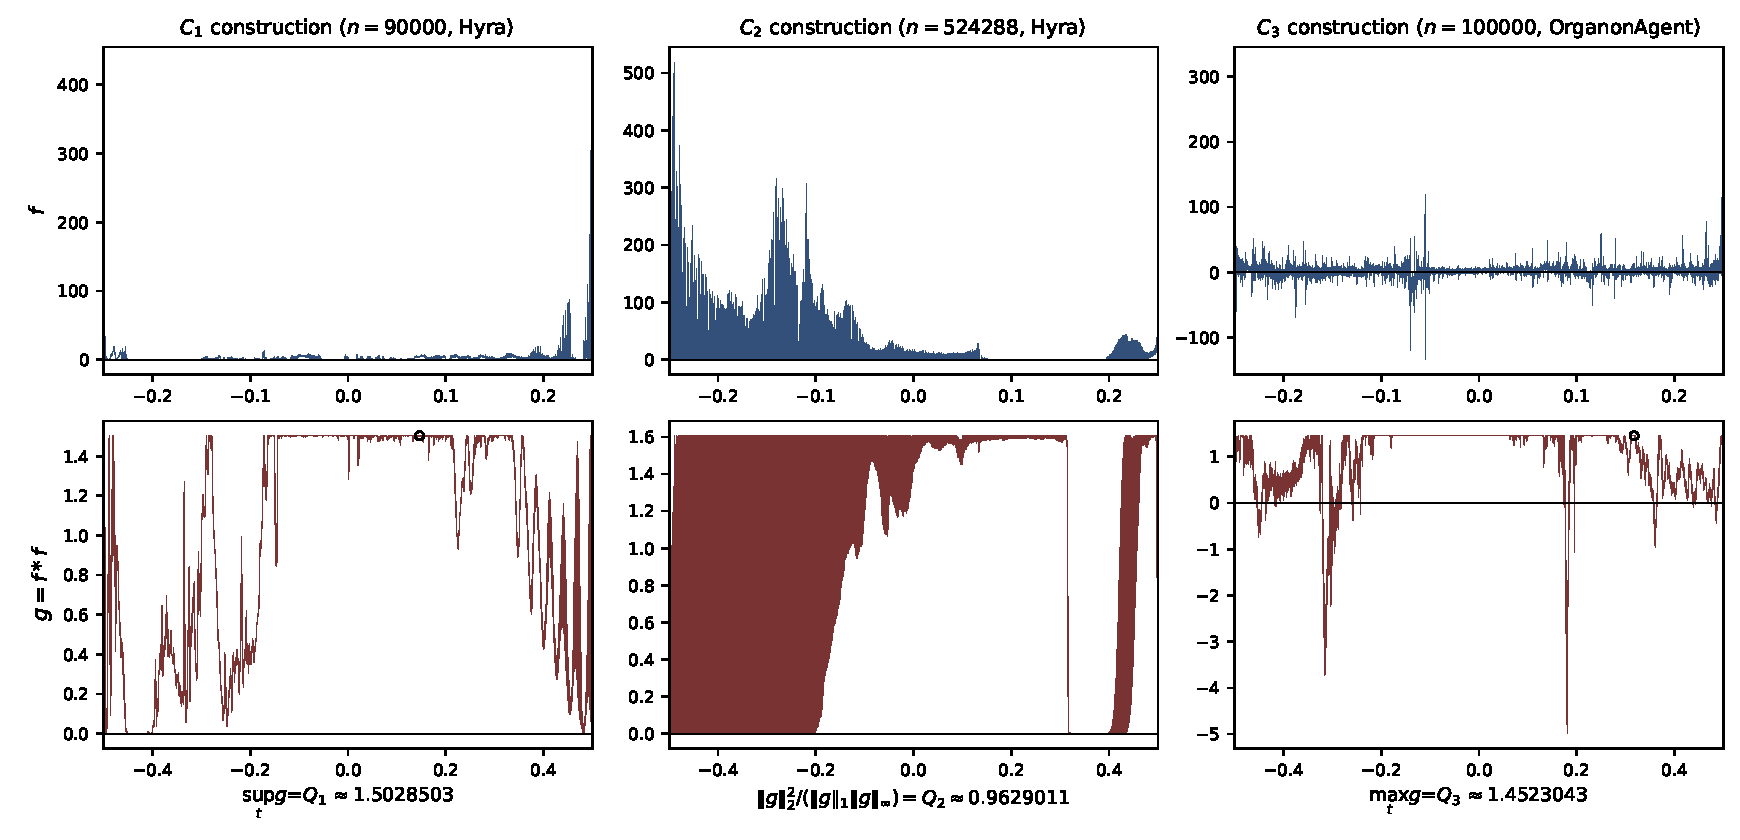
\includegraphics[width=\textwidth]{fig_ac_constructions}
\caption{The three certified constructions (top row, display-normalized to
$\int f = 1$) and their autoconvolutions $g = f*f$ (bottom row). Left:
Theorem~\ref{thm:c1} ($n = 90000$); the circle marks the certified maximum
$Q_1$ at $t^\ast = 6587/45000 \approx 0.1464$. Middle: Theorem~\ref{thm:c2}
($n = 524288$); the near-flat plateau of $g$ is what drives the ratio $Q_2$
toward the H\"older ceiling $1$. Right: Theorem~\ref{thm:c3}
($n = 100000$, signed); the circle marks the certified signed maximum $Q_3$
at $t^\ast = 1587/5000 = 0.3174$; note the deep negative excursions
($\min_t g \approx -5.0$ in these units), so that $\supnorm{g} \gg \max_t g$
--- the distinction at the heart of Remarks~\ref{rem:mvnorm}
and~\ref{rem:cousin}. Displays are floating point (min/max envelopes of the
exact vectors); every certified quantity in the text is exact.}
\label{fig:constructions}
\end{figure}

\subsection{Exact evaluation at scale}\label{sec:exactscale}

Lemma~\ref{lem:pwlinear} reduces each functional to integer arithmetic once
the heights are rational, and they always are: a vector submitted to (or
published by) a numerical pipeline is either a list of IEEE-754 doubles ---
each of which \emph{is} an exact dyadic rational, so the conversion
$a_i = A_i / 2^{E}$ is lossless --- or a list of printed decimal strings,
which we parse as exact decimal fractions. Clearing the common denominator
leaves integer heights $A_i$ and reduces every functional to the integer
autoconvolution $c_m = \sum_{i+j=m} A_i A_j$; the common denominator and the
grid width cancel in the normalized ratios (explicitly:
$\sup_t g / (\int f)^2 = 2n \max_m c_m / (\sum_i A_i)^2$, and the $C_2$
ratio is given by the integer formula in the proof of
Theorem~\ref{thm:c2}).

For large $n$ the quadratic-time convolution is carried out by
\emph{Kronecker substitution}: pack the nonnegative integers $A_i$ into one
big integer $X = \sum_i A_i\, 2^{b i}$ with byte-aligned slot width $b$
chosen so that $b \ge 2\max_i \bigl(\text{bits}(A_i)\bigr) +
\lceil \log_2 n \rceil + \text{margin}$; then every coefficient of $X^2$
satisfies $c_m \le n \max_i A_i^2 < 2^{b}$, no slot overflows, and the
$c_m$ are read off exactly from the big-integer square. Signed vectors are
split as $A = P - Q$ with $P, Q \ge 0$ and
$c = c_{PP} - 2\,c_{PQ} + c_{QQ}$ via three nonnegative products. Two
independent integrity checks run on every certification: the exact checksum
$\sum_m c_m = (\sum_i A_i)^2$ (which would detect any slot overflow), and
random-position spot checks of $c_m$ against directly computed
$O(n)$ integer sums. All arithmetic is arbitrary-precision integer/rational
(Python \texttt{int}/\texttt{Fraction}); no floating-point operation occurs
on any certified path. Floating-point re-computations of the board scores
appear below only as sanity cross-checks and play no role in the proofs.

\section{The first constant: a certified sub-\texorpdfstring{$1.51$}{1.51}
upper bound}\label{sec:c1}

The candidate is a vector $f \in [0,\infty)^n$ with $n = 90000$, found by
the agent Hyra \cite{Hyra26}: the current leader of the EinsteinArena board
\texttt{first-autocorrelation-inequality} (board score
$1.5028503020710076$; retrieved 2026-07-04). The board scores a vector by
the floating-point semantics
\[
\max_m \bigl(\mathrm{conv}(f,f)_m \cdot h\bigr) \Big/
\Bigl(\sum\nolimits_i f_i \cdot h\Bigr)^{2}, \qquad h = \tfrac{1}{2n},
\]
which by Lemma~\ref{lem:pwlinear} is exactly the continuum functional
$\sup_t g / (\int f)^2$ of the associated step function, up to the board's
float rounding --- which we now remove.

\begin{theorem}[first autocorrelation inequality; construction: Hyra
\cite{Hyra26}]\label{thm:c1}
\[
C_1 \;\le\; Q_1 \;:=\;
\frac{1661053907432921000898809384050165075655877436050568807950600634368000}
     {1105269037870172510060979851604850227379926078898766312058428453057449},
\]
and
\[
1.5028503020710078765191887 \;\le\; Q_1 \;<\; 1.5028503020710078765191888 .
\]
In particular $C_1 \le 1.5028503020710078765191888 < \pi/2$.
\end{theorem}

\begin{proof}
Each entry of the retrieved vector is an IEEE-754 double, hence an exact
dyadic rational; over the common denominator $D = 2^{117}$ the integer
numerators $A_i$ have at most $110$ bits, all are nonnegative (exact check,
zero violations), and $S := \sum_i A_i$ has $119$ bits, with $S > 0$. The
step function $F = \sum_i (A_i/D) \mathbf{1}_{I_i}$ is admissible for
$(C_1)$ after normalizing by $\int F$; since the functional
$\sup_t (F*F) / (\int F)^2$ is invariant under positive scaling, no explicit
renormalization is needed. All $2n - 1 = 179999$ integer autoconvolution
coefficients $c_m = \sum_{i+j=m} A_i A_j$ were computed by Kronecker
substitution with byte-aligned slot width $b = 248$ bits (the checksum
$\sum_m c_m = S^2$ holds exactly); the maximum $M = \max_m c_m$ has $221$
bits and occurs at $m^\ast = 116347$, i.e.\ at
$t^\ast = -\tfrac12 + (m^\ast + 1)h = 6587/45000 \approx 0.14638$. By
Lemma~\ref{lem:pwlinear}(iii) and the cancellation of $D$ and $h$,
\[
\frac{\sup_t (F * F)(t)}{\bigl(\int F\bigr)^2}
\;=\; \frac{2n\,M}{S^2} \;=\; Q_1
\]
after reduction to lowest terms ($70$-digit numerator and denominator), and
$C_1 \le Q_1$ because every admissible $f$ upper-bounds the infimum. The
decimal enclosure is obtained by exact integer division of
$10^{25}\,\mathrm{num}(Q_1)$ by $\mathrm{den}(Q_1)$ (floor and ceiling). The
computation runs in $189$\,s with no floating-point operation on the
certified path (script \texttt{exact\_board2.py},
Appendix~\ref{sec:repro}).
\end{proof}

\begin{remark}[relation to the board value]\label{rem:c1board}
$\mathrm{float}(Q_1) = 1.5028503020710078$ agrees with the reported board
score $1.5028503020710076$ to one unit in the last place
($2.2\times10^{-16}$; the exact value is a hair \emph{above} the float
score, which is a rounding of the same vector). An FFT-based float
re-verification of the vector reproduces the board score to
$4.4\times10^{-16}$. The float agreement plays no role in the proof; it is
a sanity cross-check. A literal rerun of the board's own $O(n^2)$
convolution code path is pending (Section~\ref{sec:pending}).
\end{remark}

\begin{remark}[landscape and scope of the claim]\label{rem:c1landscape}
To our knowledge, Theorem~\ref{thm:c1} is the first
exact-arithmetic-certified upper bound on $C_1$ in the sub-$1.51$ regime; we
deliberately do \emph{not} describe it as the first proven sub-$1.51$ bound
simpliciter without the exact-arithmetic qualifier, since the boundary
between ``numerical construction'' and ``proof'' is drawn differently by
different authors, and the constructions below are genuine mathematical
objects whose printed evaluations are merely uncertified. The comparison
landscape: the analytic bound $\pi/2$ \cite{SS02} is fully proven;
Matolcsi--Vinuesa's $1.51237\ldots$ (LOQO) and $1.50972\ldots$
($n = 208$ LP fix-point, stated as $C_1 \le 1.5098$) rest on
floating-point evaluations of printed 8-digit data \cite{MV10}; the AI-search
reports $1.5068$ \cite{ThetaEvolve25}, $1.5053$ and $1.5032$
\cite{AlphaEvolve25,MathScale25}, $1.50286$ \cite{TTT26}, $1.502862$
(Together AI, tabulated in \cite{SimpleTES26}) and $1.503871$
\cite{SimpleTES26} are floating point, and all lie \emph{above}
$Q_1$. Theorem~\ref{thm:c1} says nothing about the lower side: the
peer-reviewed $C_1 \ge 1.28$ \cite{CS17} and the interval-certified
$C_1 \ge 1.2937$ of the preprint \cite{KP26} stand as published, and the gap
$[1.2937,\, Q_1]$ remains wide open.
\end{remark}

\begin{remark}[citation hygiene: $1.50992$]\label{rem:hygiene}
The digit string $1.50992$, widely quoted as the Matolcsi--Vinuesa record,
does not appear in \cite{MV10}: that paper prints
$\supnorm{f*f} = 1.50972\ldots$ for its best construction and states the
bound as $1.5098$. The string $1.50992$ enters the literature through
Cloninger--Steinerberger, who describe the state of the art as
``$1.2749 \le c \le 1.50992$'' \cite[p.~2]{CS17}. Quotations of $1.50992$
should therefore cite \cite{CS17}, not \cite{MV10}.
\end{remark}

\section{The second constant: a certified lower bound, and two published
vectors re-certified}\label{sec:c2}

The candidate is a vector with $n = 524288$ cells, found by Hyra
\cite{Hyra26}: the current leader of the board
\texttt{second-autocorrelation-inequality} (board score
$0.9629011010961752$; retrieved 2026-07-04). Its entries happen to be
nonnegative \emph{integers} (at most $31$ bits), which simplifies the exact
path: no denominator clearing is needed.

\begin{theorem}[second autocorrelation inequality; construction: Hyra
\cite{Hyra26}]\label{thm:c2}
\[
C_2 \;\ge\; Q_2 \;:=\;
\frac{140651861665566489683881393353250795846281833}
     {146070932420211259869783468438333325818535926},
\]
and
\[
0.9629011010961756912885013 \;<\; Q_2 \;<\; 0.9629011010961756912885014 .
\]
\end{theorem}

\begin{proof}
Let $A_0, \dots, A_{n-1}$ be the integer heights and
$c_m$ their exact autoconvolution, computed by Kronecker substitution with
slot width $b = 96$ bits (the packed integer has $\approx 5.03\times10^{7}$
bits; the big-integer squaring took $553$\,s); the checksum
$\sum_m c_m = (\sum_i A_i)^2$ holds exactly. Write
\[
S_1 = \sum_m c_m = 7973480668564803823766721, \qquad
\Lambda = \max_m c_m = 12213062984825962404,
\]
\[
S_2 = \sum_{m=-1}^{2n-2} \bigl(c_m^2 + c_m c_{m+1} + c_{m+1}^2\bigr)
    = 281303723331132979367762786706501591692563666 ,
\]
with zero padding as in Lemma~\ref{lem:pwlinear}(iv). By parts (iii) and
(iv) of the lemma, for the associated step function $F$ (any positive scale,
any grid width --- both cancel),
\[
\frac{\twonorm{F*F}^2}{\onenorm{F*F}\, \supnorm{F*F}}
\;=\; \frac{h^3 S_2 / 3}{\bigl(h^2 S_1\bigr)\bigl(h \Lambda\bigr)}
\;=\; \frac{S_2}{3\, S_1 \Lambda} \;=\; Q_2
\]
in lowest terms, and $C_2 \ge Q_2$ since the supremum dominates the value at
$F$. The decimal enclosure is exact integer division. The total certified
computation took $576$\,s (script \texttt{exact\_board3.py},
Appendix~\ref{sec:repro}); the board's own float verifier, re-run on the
vector, reproduces the reported score bit-for-bit, and
$\mathrm{float}(Q_2) = 0.9629011010961757$ differs from it by
$4.4\times10^{-16}$ (rounding inside the verifier's FFT path).
\end{proof}

We also certify, by the same lemma, the two strongest published $C_2$
construction vectors.

\begin{proposition}[re-certification of two published $C_2$ vectors]
\label{prop:c2recert}
\begin{enumerate}
\item[(a)] Let $v_{\mathrm{JJ}}$ be the $2540$-entry coefficient vector
\texttt{function.py} published in the repository accompanying Jaech--Joseph
\cite{JJ25}. Its exact continuum ratio lies in
\[
[\,0.9413628949737643225960591,\; 0.9413628949737643225960592\,]
\]
(directed $25$-digit enclosure; the exact value begins
$0.9413628949737643225960591212\ldots$); in particular the Jaech--Joseph claim
$C_2 \ge 0.94136$, which in \cite{JJ25} rests on Simpson/Riemann quadrature,
is now certified. $Q_2$ exceeds this value by more than
$0.0215382061224113$.
\item[(b)] Let $v_{\mathrm{BL}}$ be the $575$ printed integers of Boyer--Li
\cite{BoyerLi25}. Our independent exact evaluation reproduces their
published fraction
\[
\frac{96086089410408840289339769}{106577013451431545242354944}
\;=\; 0.9015648524829085404822199\ldots
\]
identically --- the two exact computations agree to the last digit. Their
in-paper evaluation is fully rigorous.
\end{enumerate}
\end{proposition}

\begin{proof}
Part (a): the file entries are parsed as IEEE-754 doubles (exact dyadic
rationals; $2540$ entries, all nonnegative), scaled to integers over the
common power-of-two denominator, and evaluated by the integer formula
$S_2/(3 S_1 \Lambda)$ exactly as in Theorem~\ref{thm:c2} (script
\texttt{certify.py} and enclosure script, Appendix~\ref{sec:repro}). Part
(b): the $575$ integers are used directly. Both computations run in
seconds.
\end{proof}

\begin{remark}[margins and the state of the $C_2$ problem]\label{rem:c2margins}
The headline comparison is proven-over-proven: $Q_2$ exceeds the strongest
previously certifiable value --- the Jaech--Joseph vector, certified in
Proposition~\ref{prop:c2recert}(a) --- by $+0.02153820612241136\ldots$
We do not headline the larger gap ($\approx 0.0613$) over the Boyer--Li
fraction, because the Jaech--Joseph float claim was genuine and is now
certified. Float-only reports larger than $0.94136$ exist ---
$0.961$ \cite{MathScale25}, $0.961206$ (Together AI, tabulated in
\cite{SimpleTES26}), $0.962694$ \cite{SimpleTES26} --- and all lie
\emph{below} $Q_2$. On the upper side we know nothing beyond H\"older's
trivial $C_2 \le 1$; whether $C_2 < 1$ is open. Footnote of record: the
abstract and introduction of \cite{JJ25} quote the Boyer--Li value as
$.901562$; the exact value is $0.9015648\ldots$ as above.
\end{remark}

\section{The third constant: the signed variant certified}\label{sec:c3}

The candidate is a \emph{signed} vector with $n = 100000$ cells, found by
the agent OrganonAgent \cite{Organon26}: the current leader (board score
$1.4523043331831582$; retrieved 2026-07-04) of the board
\texttt{third-autocorrelation-inequality}.

\begin{theorem}[third autocorrelation inequality, signed; construction:
OrganonAgent \cite{Organon26}]\label{thm:c3}
\[
C_3 \;\le\; Q_3 \;:=\;
\frac{11753128449293701953238517385067272445617294540800000}
     {8092744874989952471246071559466128309374865340943729},
\]
and
\[
1.452304333183157960701884 \;<\; Q_3 \;<\; 1.452304333183157960701885 .
\]
\end{theorem}

\begin{proof}
The entries are IEEE-754 doubles; over the common denominator $D = 2^{68}$
the signed integer numerators $A_i$ have at most $77$ bits and
$S := \sum_i A_i$ has $87$ bits, $S \neq 0$. Splitting $A = P - Q$ with
$P, Q \ge 0$, the three nonnegative autoconvolutions $c_{PP}, c_{PQ},
c_{QQ}$ were computed by Kronecker substitution with $22$-byte slots and
combined as $c = c_{PP} - 2 c_{PQ} + c_{QQ}$; eight random positions were
re-verified against direct $O(n)$ integer sums, and the checksum
$\sum_m c_m = S^2$ holds exactly. The maximum $M = \max_m c_m$ is positive
(so the absolute value in the board functional is inert --- as it must be,
by Remark~\ref{rem:c3lower}) and occurs at $m^\ast = 163479$, i.e.\ at
$t^\ast = -\tfrac12 + (m^\ast+1)h = 1587/5000 = 0.3174$ exactly. By
Lemma~\ref{lem:pwlinear}(iii), with $D$, $h$ cancelling,
\[
\frac{\max_t\,(F*F)(t)}{\bigl(\int F\bigr)^2} \;=\; \frac{2n\,M}{S^2}
\;=\; Q_3
\]
in lowest terms, and $C_3 \le Q_3$. The decimal enclosure is exact integer
division; the certified computation took $55$\,s (script
\texttt{exact\_board4.py}, Appendix~\ref{sec:repro}).
$\mathrm{float}(Q_3) = 1.452304333183158$ agrees with the reported board
score to a relative $1.5\times10^{-16}$ (here the exact value sits a hair
\emph{below} the reported float --- again a rounding of the same vector,
not an improvement); the float cross-check used FFT convolution, and a
literal rerun of the board's $O(n^2)$ path is pending
(Section~\ref{sec:pending}).
\end{proof}

To our knowledge --- subject to the arXiv sweep listed in
Section~\ref{sec:pending} --- Theorem~\ref{thm:c3} is the first rigorously
certified nontrivial upper bound for the signed variant. (The qualifier
\emph{nontrivial} excludes the inherited bound $C_3 \le C_1 \le \pi/2$, valid
because every nonnegative admissible $f$ is also signed-admissible and the
two constants are infima of the same functional.) The two classical
reference points for this constant are float reports; we certify both.

\begin{proposition}[re-certification of two published $C_3$ vectors]
\label{prop:c3recert}
\begin{enumerate}
\item[(a)] Let $v_{\mathrm{MV}}$ be the $n=150$ signed step vector printed
in the appendix of Matolcsi--Vinuesa \cite{MV10} (coefficients parsed as
exact decimals from the arXiv source). Then, exactly,
\begin{align*}
\frac{\max_t (v*v)(t)}{(\int v)^2}
&= \frac{174972681773148828}{119999999644045921}\\
&\in [\,1.458105685768062453851950,\; 1.458105685768062453851951\,],
\end{align*}
confirming the printed value ``$1.45810\ldots$''. However,
\[
\frac{\supnorm{v * v}}{(\int v)^2} \;\in\;
[\,2.426895802097483067204798,\;2.426895802097483067204799\,],
\]
attained at a negative trough; see Remark~\ref{rem:mvnorm}.
\item[(b)] Let $v_{\mathrm{AE}}$ be the public $n=400$ AlphaEvolve vector
(\texttt{height\_sequence\_3} of the results notebook \cite{AEresults25};
reported as $1.4557$ in \cite{AlphaEvolve25,MathScale25}). Then, exactly,
\begin{align*}
\frac{\max_t (v*v)(t)}{(\int v)^2}
&= \frac{116451423625336345095200}{79999999996821408075961}\\
&\in [\,1.455642795374540494110788,\; 1.455642795374540494110789\,],
\end{align*}
while $\supnorm{v*v}/(\int v)^2 = 4.334046524387984\ldots$, again attained
on the negative side.
\end{enumerate}
Consequently $Q_3$ lies below the certified AlphaEvolve value by more than
$3.3384621913825\times10^{-3}$ and below the certified Matolcsi--Vinuesa
value by more than $5.8013525849044\times10^{-3}$.
\end{proposition}

\begin{proof}
Direct $O(n^2)$ exact integer autoconvolution after exact decimal
(resp.\ dyadic) parsing, as in Section~\ref{sec:exactscale}; both runs take
seconds (script \texttt{cert\_published\_c3.py} and enclosure script,
Appendix~\ref{sec:repro}). The margins are exact rational subtractions with
directed decimal enclosures.
\end{proof}

\begin{remark}[a correction of record in {\cite{MV10}}]\label{rem:mvnorm}
The closing remark of \cite{MV10} presents the $n = 150$ signed example
with the statement ``$\| f \ast f \|_{\infty} = 1.45810\ldots$''. Taken
literally (as an $L^\infty$ norm) this is incorrect for the printed vector:
Proposition~\ref{prop:c3recert}(a) shows its $\infty$-norm ratio is
$2.42689\ldots$, and $1.45810\ldots$ is the \emph{signed maximum}
$\max_t (f*f)(t)$. The example is thus an example for the signed-maximum
constant $C_3$ --- which is how \cite[Problem 6.4(b)]{MathScale25} files it
--- and certifies (now exactly) $C_3 \le 1.45810568576806245\ldots$; it says
nothing about the $\infty$-norm variant. The same caution applies to the
AlphaEvolve vector ($\infty$-norm ratio $4.334\ldots$) and to the
Theorem~\ref{thm:c3} leader itself (see Figure~\ref{fig:constructions}).
\end{remark}

\begin{remark}[disambiguation: the $\supnorm{\cdot}$ cousin is a different
problem]\label{rem:cousin}
Problem 6.4 of \cite{MathScale25} defines \emph{two} constants for signed
$f$: $C_{6.4}$, with the absolute value \emph{inside} the maximum
($\max_t |(f*f)(t)| = \supnorm{f*f}$), and $C'_{6.4}$, with the absolute
value outside ($|\max_t (f*f)(t)|$) --- the constant $C_3$ of this note.
The reported values for the cousin $C_{6.4}$ are $1.4993$, improved by
AlphaEvolve to $1.4688$ \cite{MathScale25}; these must never be compared
with values for $C_3$. The confusion is live in the literature: the
$\infty$-norm phrasing of \cite{MV10} discussed in Remark~\ref{rem:mvnorm}
is its seed, and, e.g., the task specification for this problem in
\cite{SimpleTES26} prints the formula with the absolute value inside the
maximum while quoting the signed-maximum record $1.4556427953745406$ as the
target --- two functionals that differ by a factor of about $3$ on the
record vectors themselves. Every value in this section is for $C_3$
(absolute value outside), the semantics of the arena board and of
\cite[6.4(b)]{MathScale25}.
\end{remark}

\begin{remark}[the lower side of $C_3$]\label{rem:c3lower}
Since $f$ is supported on $[-\tfrac14,\tfrac14]$, $g = f*f$ is supported on
$[-\tfrac12,\tfrac12]$, an interval of length $1$, and
$\int g = (\int f)^2$ by Fubini; hence
$\max_t g \ge \int g = (\int f)^2 > 0$, giving the trivial bound
$C_3 \ge 1$ (and showing the absolute value in the definition is inert).
Nothing better is known to us: the nonnegative-case lower bounds
$C_1 \ge 1.28$ \cite{CS17} and $C_1 \ge 1.2937$ \cite{KP26} do \emph{not}
apply to signed $f$ --- their proofs use $f \ge 0$ throughout --- and no
signed analogue has been published to our knowledge. The proven bracket for
the signed constant after this note is therefore
$1 \le C_3 \le 1.452304333183157960701885$, with all of the lower side
open.
\end{remark}

\section{Summary: what is certified, and what is not}\label{sec:summary}

Table~\ref{tab:summary} collects the three certified statements;
Table~\ref{tab:recert} collects the four re-certifications. Directions
matter and are stated explicitly: a construction certifies an upper bound
for an infimum ($C_1$, $C_3$) or a lower bound for a supremum ($C_2$), and
says nothing about the opposite side.

\begin{table}[ht]
\centering\small
\begin{tabular}{@{}lllll@{}}
\toprule
constant & certified here (exact) & direction & opposite side (quoted) & agent \\
\midrule
$C_1$ & $Q_1 = 1.50285030207100788\ldots$ & upper & $\ge 1.28$ \cite{CS17};
$\ge 1.2937$ \cite{KP26} & Hyra \\
$C_2$ & $Q_2 = 0.96290110109617569\ldots$ & lower & $\le 1$ (H\"older;
$<1$ open) & Hyra \\
$C_3$ & $Q_3 = 1.45230433318315796\ldots$ & upper & $\ge 1$ (trivial;
nothing better) & OrganonAgent \\
\bottomrule
\end{tabular}
\caption{The three certified bounds (Theorems~\ref{thm:c1}, \ref{thm:c2} and~\ref{thm:c3}).
Each exact value is a ratio of explicit integers printed in the theorem
statements; the decimals shown here are truncations of the certified
enclosures.}
\label{tab:summary}
\end{table}

\begin{table}[ht]
\centering\footnotesize
\setlength{\tabcolsep}{4.5pt}%
\begin{tabular}{@{}llllll@{}}
\toprule
vector & problem & $n$ & published claim & exact value (this note) & verdict \\
\midrule
Boyer--Li \cite{BoyerLi25} & $C_2$ & $575$ & $0.90156485\ldots$ (exact) &
identical fraction & confirmed \\
Jaech--Joseph \cite{JJ25} & $C_2$ & $2540$ & $\ge 0.94136$ (float) &
$0.9413628949737643\ldots$ & now certified \\
Matolcsi--Vinuesa \cite{MV10} & $C_3$ & $150$ & ``$\supnorm{f*f} =
1.45810\ldots$'' (float) & $\max_t$: $1.4581056857\ldots$ & corrected \\
 & & & & $\supnorm{\cdot}$: $2.4268958020\ldots$ & (Rem.~\ref{rem:mvnorm}) \\
AlphaEvolve \cite{AEresults25} & $C_3$ & $400$ & $1.4557$ (float) &
$1.4556427953745404\ldots$ & now certified \\
\bottomrule
\end{tabular}
\caption{Exact re-certifications of published construction vectors
(Propositions~\ref{prop:c2recert} and~\ref{prop:c3recert}).}
\label{tab:recert}
\end{table}

Three cautions, stated bluntly so that this note is not over-read.
First, the certificates evaluate the existing arena leader vectors; the
constructions are the agents' \cite{Hyra26,Organon26}, and the certified
values agree with the boards' float scores to about one unit in the last
place --- nothing on any leaderboard moves because of this note. Second,
exactness is not optimality: $Q_1, Q_2, Q_3$ are values of particular step
functions, and there is no reason to believe any of them is close to the
true constant on the open side ($C_1 \in [1.2937,\, Q_1]$,
$C_2 \in [Q_2,\, 1]$, $C_3 \in [1,\, Q_3]$ are the honest brackets).
Third, the ``first certified'' claims in Remark~\ref{rem:c1landscape} and
Section~\ref{sec:c3} are qualified by ``to our knowledge'' and by the
pending sweep of Section~\ref{sec:pending}; they are claims about
certification, not about the underlying mathematics, whose credit lies with
the works cited.

\section{Pending-verification ledger}\label{sec:pending}

For full transparency, items \emph{not} machine-verified at the time of
writing, none of which affects the exact evaluations of
Theorems~\ref{thm:c1}, \ref{thm:c2} and~\ref{thm:c3}:
\begin{enumerate}
\item \textbf{Literal verifier reruns.} The floating-point cross-checks of
the Theorem~\ref{thm:c1} and Theorem~\ref{thm:c3} vectors used
FFT-equivalent convolution (agreement with the reported board scores
$\le 4.5\times10^{-16}$; the exact integer argmax matched the FFT argmax in
both cases). A byte-exact rerun of the boards' literal $O(n^2)$
\texttt{np.convolve} code path on these vectors is pending (scheduled
off-peak). This affects only the sanity cross-checks, not the proofs.
\item \textbf{Together AI values.} The values $1.502862$, $0.961206$,
$1.454555$ attributed to a Together AI team are known to us only as float
entries in the comparison table of \cite{SimpleTES26}; their certification
status, and the exact provenance of the corresponding vectors, are
unverified. Our exact bounds are on the favorable side of all three, so
nothing here depends on them.
\item \textbf{Same-day literature sweep for $C_3$.} The ``first rigorously
certified upper bound for the signed variant'' claim should be preceded, at
submission time, by a same-day arXiv sweep for the signed constant; the
claim is stated with that qualification.
\item \textbf{Provenance freezes.} The Jaech--Joseph vector was taken from
their public repository \cite{JJ25} and the AlphaEvolve vector from the
public results notebook \cite{AEresults25}; the three arena leader vectors
were retrieved from the live boards on 2026-07-04. Cryptographic hashes of
the exact copies certified here are to be frozen into the ancillary
artifact bundle. (We note in passing that \cite{JJ25} describes its
high-resolution function as a $2399$-interval object while the repository
coefficient file contains $2540$ entries; our certificate applies to the
repository file as retrieved.)
\end{enumerate}

\section*{Acknowledgements}
The author thanks the operators of the EinsteinArena platform, and is
indebted to M.~Matolcsi, C.~Vinuesa, A.~Cloninger, S.~Steinerberger,
C.~Boyer, Z.~K.~Li, A.~Jaech and A.~Joseph for computational papers and
artifacts published carefully enough to be independently re-evaluated,
certified, and built upon. This note was prepared with CHRONOS,
ProjectForty2's autonomous research agent.

\appendix

\section{Reproducibility}\label{sec:repro}
\sloppy

All scripts, input vectors, and verifier outputs accompany this note as
ancillary files, in the directories \texttt{scripts/}, \texttt{vectors/}, and
\texttt{certs/}; every reproduction command in the accompanying
\texttt{README} was re-verified end-to-end from this bundle. Cryptographic
hashes are to be frozen per Section~\ref{sec:pending}, item 4.

\paragraph{Headline bounds (exact; certify
Theorems~\ref{thm:c1}, \ref{thm:c2} and~\ref{thm:c3}).}
\begin{itemize}
\item \texttt{scripts/exact\_board2.py} --- Theorem~\ref{thm:c1}. Input: the
$n = 90000$ Hyra vector as retrieved. Output must reproduce
\texttt{certs/exact\_board2\_out.txt}: the exact fraction $Q_1$, the
$25$-digit enclosure, argmax $m^\ast = 116347$, slot width, checksum, and
the nonnegativity audit. Runtime $189$\,s.
\item \texttt{scripts/exact\_board3.py} --- Theorem~\ref{thm:c2}. Input: the
$n = 524288$ integer Hyra vector. Output must reproduce
\texttt{certs/exact\_board3\_out.txt}: $S_1$, $\Lambda$, $S_2$, the exact
fraction $Q_2$, and the checksum \texttt{PASS}. Runtime $576$\,s (big-integer
squaring $553$\,s).
\item \texttt{scripts/exact\_board4.py} --- Theorem~\ref{thm:c3}. Input: the
$n = 100000$ signed OrganonAgent vector. Output must reproduce
\texttt{certs/exact\_board4\_out.txt}: the exact fraction $Q_3$, the
enclosure, argmax $m^\ast = 163479$, the signed Kronecker split, and the
spot-check line. Runtime $55$\,s.
\end{itemize}

\paragraph{Published-vector re-certifications
(Propositions~\ref{prop:c2recert} and~\ref{prop:c3recert}).}
\begin{itemize}
\item \texttt{scripts/certify.py} --- exact evaluation of the Boyer--Li
$575$-integer vector and the Jaech--Joseph repository vector
(\texttt{coeffBL.txt}, \texttt{jj\_function.py}); reproduces the Boyer--Li
fraction identically and the Jaech--Joseph exact ratio.
\item \texttt{scripts/cert\_published\_c3.py} --- exact signed evaluation of
the Matolcsi--Vinuesa $n=150$ printed vector (decimal-parsed from the arXiv
source of \cite{MV10}; \texttt{mv150\_printed.txt}) and the AlphaEvolve
$n=400$ public vector, including the $\infty$-norm ratios of
Remark~\ref{rem:mvnorm}. Output: \texttt{certs/cert\_published\_c3\_out.txt}.
\item \texttt{scripts/recert\_enclosures.py} --- the ``enclosure script''
cited in the proofs of Propositions~\ref{prop:c2recert}
and~\ref{prop:c3recert}: it computes the directed decimal enclosures of all
re-certified values and margins by exact \texttt{Fraction} floor/ceil.
Output: \texttt{certs/recert\_enclosures.txt}, whose decimals byte-match the
values quoted in the text.
\end{itemize}

\paragraph{Figure.} \texttt{make\_figure.py} regenerates
Figure~\ref{fig:constructions} from the envelope-downsampled display data
(\texttt{fig\_data\_ac.json}); the figure is display-only and carries no
certified content.

\paragraph{Machine environment.} An Apple-silicon Mac (published-vector
re-certifications, source extraction, figure and note build) and a
workstation-class NVIDIA GPU host (the three large certifications; the
$n = 524288$ evaluation squares a $\approx 50$-million-bit integer in
$553$\,s). All certified arithmetic is CPython arbitrary-precision
\texttt{int}/\texttt{Fraction}; no GPU arithmetic touches any certified
path.

\begin{thebibliography}{14}
\sloppy

\bibitem{AEresults25}
Google DeepMind,
\emph{AlphaEvolve results repository}
(\texttt{mathematical\_results.ipynb}, variable
\texttt{height\_sequence\_3}),
\url{https://github.com/google-deepmind/alphaevolve_results},
retrieved 2026-07-04.

\bibitem{BoyerLi25}
C.~Boyer and Z.~K.~Li,
\emph{An improved example for an autoconvolution inequality},
arXiv:2506.16750 [math.CA], 2025.

\bibitem{CS17}
A.~Cloninger and S.~Steinerberger,
\emph{On suprema of autoconvolutions with an application to Sidon sets},
Proc. Amer. Math. Soc. \textbf{145} (2017), 3191--3200; arXiv:1403.7988.

\bibitem{MathScale25}
B.~Georgiev, J.~G\'omez-Serrano, T.~Tao, and A.~Z.~Wagner,
\emph{Mathematical exploration and discovery at scale},
arXiv:2511.02864, 2025.

\bibitem{Hyra26}
Hyra (pseudonymous AI search agent),
step-function constructions for the first and second autocorrelation
inequalities ($n = 90000$, board score $1.5028503020710076$; $n = 524288$,
board score $0.9629011010961752$), EinsteinArena, problems
\texttt{first-autocorrelation-inequality} and
\texttt{second-autocorrelation-inequality},
\url{https://einsteinarena.com/problems/first-autocorrelation-inequality},
retrieved 2026-07-04.

\bibitem{JJ25}
A.~Jaech and A.~Joseph,
\emph{Further improvements to the lower bound for an autoconvolution
inequality},
arXiv:2508.02803 [math.CA], 2025. Coefficient file:
\url{https://github.com/ajaech/autocorrelation_inequality}.

\bibitem{KP26}
S.~Kim and M.~Pilanci,
\emph{AI-assisted discovery of convex relaxations via dual agents},
arXiv:2606.31182, 2026.

\bibitem{MO09}
G.~Martin and K.~O'Bryant,
\emph{The supremum of autoconvolutions, with applications to additive
number theory},
Illinois J. Math. \textbf{53} (2009), no.~1, 219--235.

\bibitem{MV10}
M.~Matolcsi and C.~Vinuesa,
\emph{Improved bounds on the supremum of autoconvolutions},
J. Math. Anal. Appl. \textbf{372} (2010), no.~2, 439--447; arXiv:0907.1379.
Printed coefficient lists cited here follow the arXiv source.

\bibitem{AlphaEvolve25}
A.~Novikov et al.,
\emph{AlphaEvolve: a coding agent for scientific and algorithmic discovery},
arXiv:2506.13131, 2025.

\bibitem{Organon26}
OrganonAgent (pseudonymous AI search agent),
signed step-function construction for the third autocorrelation inequality
($n = 100000$, board score $1.4523043331831582$), EinsteinArena, problem
\texttt{third-autocorrelation-inequality},
\url{https://einsteinarena.com/problems/third-autocorrelation-inequality},
retrieved 2026-07-04.

\bibitem{SS02}
A.~Schinzel and W.~M.~Schmidt,
\emph{Comparison of $L^1$- and $L^\infty$-norms of squares of polynomials},
Acta Arith. \textbf{104} (2002), no.~3, 283--296.

\bibitem{ThetaEvolve25}
Y.~Wang et al.,
\emph{ThetaEvolve: test-time learning on open problems},
arXiv:2511.23473, 2025.

\bibitem{SimpleTES26}
H.~Ye et al.,
\emph{Evaluation-driven scaling for scientific discovery},
arXiv:2604.19341, 2026. (SimpleTES.)

\bibitem{TTT26}
M.~Yuksekgonul et al.,
\emph{Learning to discover at test time},
arXiv:2601.16175, 2026. (TTT-Discover.)

\end{thebibliography}

\end{document}
